\documentclass[10pt]{beamer}

\mode<presentation>
{
  \usetheme[height=1.25cm]{Madrid}
  \setbeamertemplate{navigation symbols}{}
  \setbeamercolor{alerted text}{fg=illini}
}

\graphicspath{{figs/}}

\usebackgroundtemplate{
\includegraphics[width=\paperwidth,height=\paperheight]{uc-background}}

\usepackage[english]{babel}
\usepackage{epsfig,subfigure,bm}
\usepackage{multimedia}
\usepackage{psfrag}
\usepackage{animate}

% \usefonttheme{metropolis} % default family is serif
%%%%%% Begin of my macros and options

\setbeamertemplate{section in toc shaded}[default][55]
\setbeamertemplate{subsection in toc shaded}[default][55]
\setbeamercolor{block title}{fg=white,bg=illini}
\setbeamercolor{block body}{fg=black,bg=mygrey}

\setbeamercolor{emphprimary}{fg=CBlue}
\setbeamercolor{emphsecondary}{fg=illini}
\setbeamercolor{emphtertiary}{fg=mygreen}
\definecolor{darkForestGreen}{rgb}{.1,1,.1}
\definecolor{veryLightGray}{rgb}{.9,.9,.9}
\definecolor{greenApple}{rgb}{.3,.9,.3}

\setbeamercolor{title}{bg=CBlue}

\usepackage{amsmath,amssymb,amsxtra,amsthm}
\usepackage{algorithm,algorithmic}
\usepackage{natbib}
\usepackage{bibentry}
\usepackage{xspace}
\usepackage{changepage}

\definecolor{myblue}{rgb}{.2,.2,.7}
\definecolor{myred}{rgb}{.7,.2,.2}
\definecolor{mygreen}{rgb}{.2,.7,.2}
\definecolor{mygrey}{rgb}{0.9,0.9,0.9}
\definecolor{CBlue}{cmyk}{1,0.25,0,0}
\definecolor{illini}{rgb}{0.98,0.4,0.05}
\definecolor{black}{cmyk}{0,0,0,1}

\newcommand{\myemph}[1]{{\usebeamercolor[fg]{emphprimary}
    \textbf{#1}}}
\newcommand{\myemphalt}[1]{{\usebeamercolor[fg]{emphsecondary}
    \textbf{#1}}}

\graphicspath{{figs/}}

\title[Math for Robotics] % (optional, use only with long paper titles)
{CSE276C - Factor Graph for Mapping and Localization}

\author[H.~I. Christensen] % (optional, use only with lots of authors)
{Henrik I.~Christensen}
% - Give the names in the same order as the appear in the paper.  -
% Use the \inst{?} command only if the authors have different
% affiliation.

\AtBeginSection[]
{
   \begin{frame}
       \frametitle{Outline}
       \tableofcontents[currentsection]
   \end{frame}
}

\institute[UCSD] % (optional, but mostly needed)
{
  \begin{minipage}[c]{.2\textwidth}
    
\includegraphics[width=.65\linewidth]{ucsealnew}%
  \end{minipage}%
  \begin{minipage}[c]{.6\textwidth}
    \small
%%    \begin{center}
      Computer Science and Engineering\\
      University of California, San Diego\\
%%    \end{center}

  \end{minipage}
%%  \vspace*{1ex}
}
%% - Use the \inst command only if there are several affiliations.
%% - Keep it simple, no one is interested in your street address.

\bigskip

\date[Nov 2024]% (optional, should be abbreviation of conference name)
{\small%
  November 2024}

\begin{document}

\nobibliography{/Users/hic/Dropbox/bibliography/bib-file}
\bibliographystyle{plain}

\begin{frame}[plain]
  \titlepage
\end{frame}

\begin{frame}
  \frametitle{Background Material}
  \begin{itemize}
    \item F. Dellaert, Factor Graphs and GTSAM: A Hands-on Introduction, GT Tech Report, 2012
    \item M. Kaess \& F. Dellaert, Factor graphs for robot perception, Foundations and Trends in Robotics, 2017. 
    \item Optional -- C. Stachniss, Graph SLAM in 90 minutes, University of Bonn. 2015.
    \item \url{https://github.com/SLAM-Handbook-contributors/slam-handbook-public-release/blob/main/main.pdf} SLAM HandBook (2024)
  \end{itemize}
\end{frame}

\section{Recap - Factor Graphs}

\begin{frame}
  \frametitle{Factor Graphs}
  \begin{columns}
    \begin{column}{4cm}
      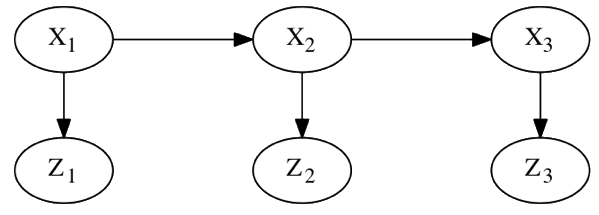
\includegraphics[width=3.9cm]{hmm}
    \end{column}
    \begin{column}{3.5cm}
      \begin{itemize}
        \item Simple HMM model for interaction
        \item Here a 1-order chain
      \end{itemize}
    \end{column}
  \end{columns}
\end{frame}

\begin{frame}
  \frametitle{Factor Graphs}
  \begin{columns}
    \begin{column}{4cm}
      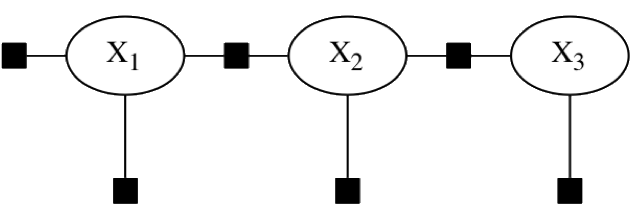
\includegraphics[width=3.9cm]{hmm-FG}
    \end{column}
    \begin{column}{3.5cm}
      \begin{itemize}
        \item Conversion to a factor graph 
        \item Nodes are functions and arcs causal links with factors that express conditional probabilities 
      \end{itemize}
    \end{column}
  \end{columns}
  \vspace{5mm} 

  \centerline{\small $P(X1,X2,X3|Z1,Z2,Z3) \propto P(X1)P(X2|X1)P(X3|X2)L(X1;z1)L(X2;z2)L(X3;z3)$}
  \vspace{5mm} 

  \centerline{\small where $L(X_t;z) \propto P(Z_t=z|Xt)$}
  \vspace{5mm} 

  \centerline{\small Our objective is maximize $f(X1,X2,X3)=\prod_i f_i(X_i)$}
\end{frame}

\section{Modeling motion}

\begin{frame}{Simple motion}
  \centerline{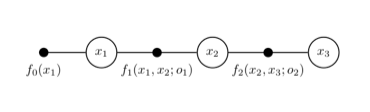
\includegraphics[width=8cm]{FactorGraph}}
  \begin{itemize}
    \item Consider a simple example of a robot moving
    \item The uniary factor $f_0(x_1)$ is our prior knowledge about initial position
    \item The binary factors $f_1(x_1, x_2; o_1)$ and $f_2(x_2, x_3, o_2)$ connect the graph where $o_i$ represents odometric measurements 
  \end{itemize}
\end{frame}


\begin{frame}{C++ implementation - Graph Initialization}
  \centerline{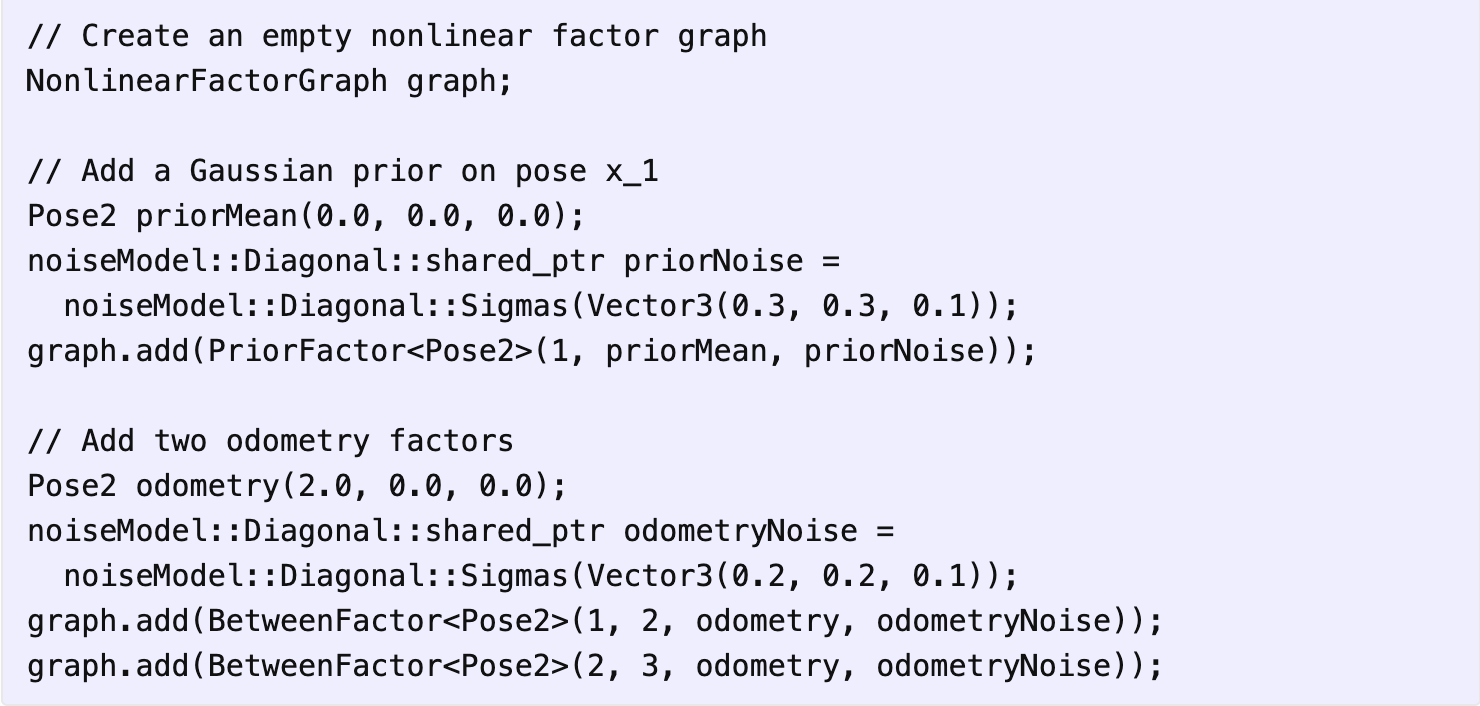
\includegraphics[width=10cm]{odometry-c++.png}}
\end{frame}

\begin{frame}{C++ implementation - Estimating a solution}
  \centerline{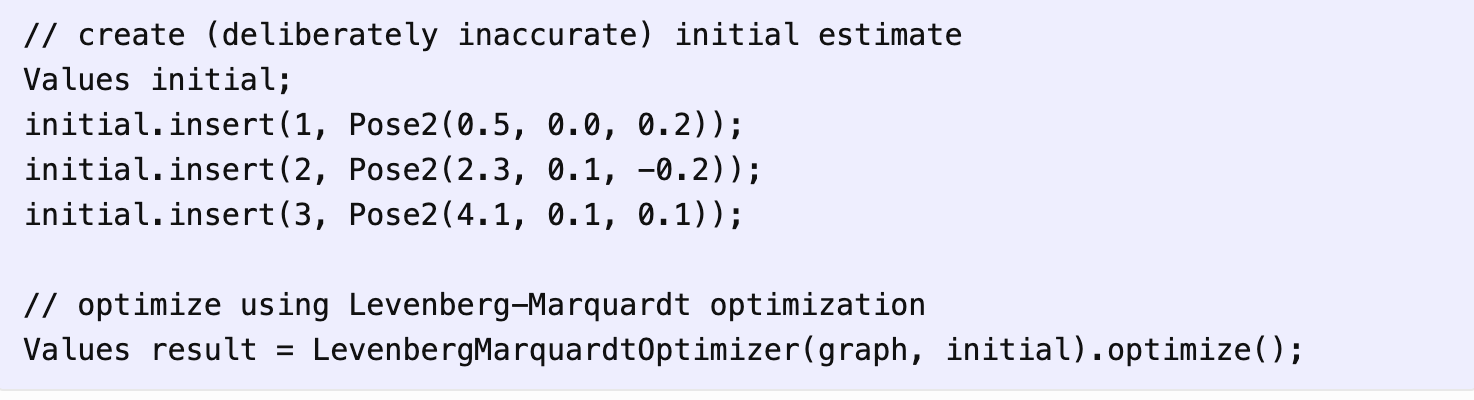
\includegraphics[width=10cm]{odometry-values.png}}
\end{frame}

\begin{frame}{C++ implementation - Results}
  \centerline{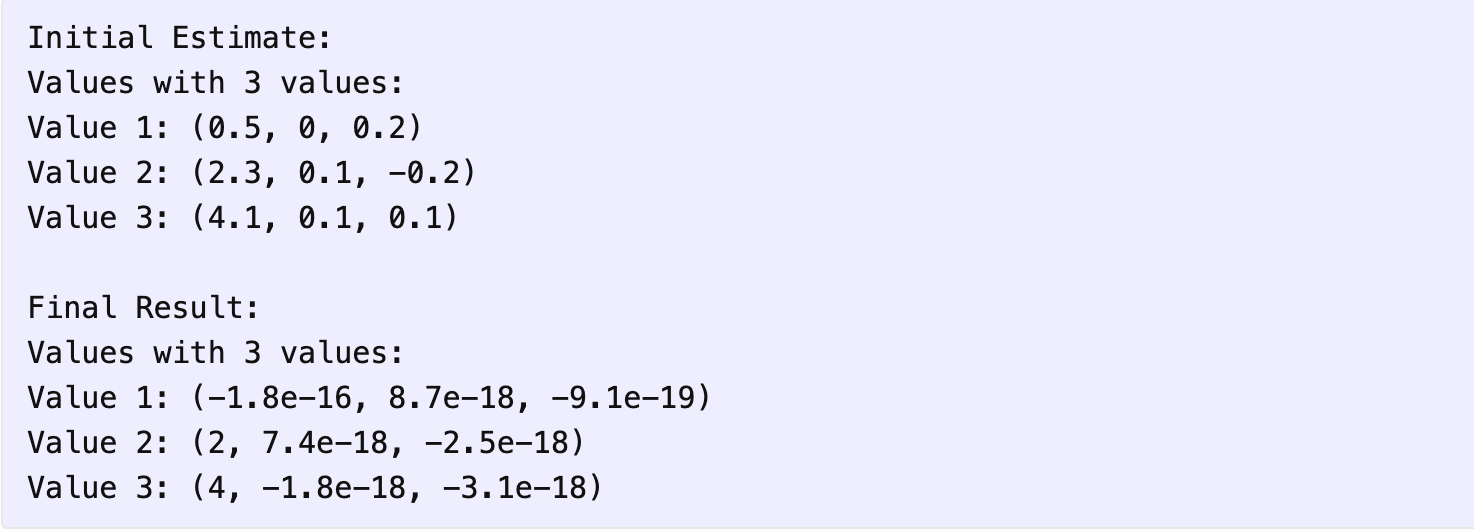
\includegraphics[width=10cm]{odometry-result.png}}
  \begin{itemize}
    \item The correct pose(s) are very well recovered
  \end{itemize}
\end{frame}

\section{Robot Localization}

\begin{frame}
  \frametitle{Localization}
  \begin{itemize}
    \item Odometry alone is not that interesting
    \item What if there are measurements of landmarks?
    \item Integration of measurements and world maps into the estimation process
    \item Assume we get a set of feature measurements - $z_i$
    \item We can model the sensors ($f_1(x_1; z_1),~ f_2(x_2; z_2)$, and $f_3(x_3; z_3)$)
  \end{itemize}
\end{frame}

\begin{frame}
  \frametitle{Setting up the network}
  \centerline{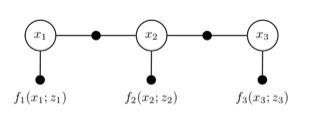
\includegraphics[width=7cm]{FactorGraph2.png}}
  \begin{itemize}
    \item We have to create customized factors for the landmark sensing
    \item We need to generate the Gaussian likelihood 
    \[
      L(q;m)= \exp \left\{-\frac{1}{2}||h(q) - m||^2_{\Sigma}\right\}=f(q)
    \] 
    where m is the measurement and h(q) is the estimate of the feature (q) in the map
  \end{itemize}
\end{frame}

\begin{frame}
  \frametitle{Computing h(q)}
  \begin{itemize}
    \item The term $h(q)$ is a projection of the feature (q) into robot coordinates. 
    \item Assume $q = (q_x, q_y, q_{\theta})^T$ 
    \item We can do a ``basic calculation''
    \[ h(q) = \left[ \begin{array}{c} q_{xr} \\ q_{yr} \end{array} \right] 
            = H q = \left[ \begin{array}{ccc} \cos(q_{\theta}) & -\sin(q_{\theta}) & 0 \\ 
                                              \sin(q_{\theta}) & \cos(q_{\theta}) & 0\end{array} \right] q 
    \]
  \end{itemize}
\end{frame}

\begin{frame}{C++ Implementation of Custom Factors}
  \centerline{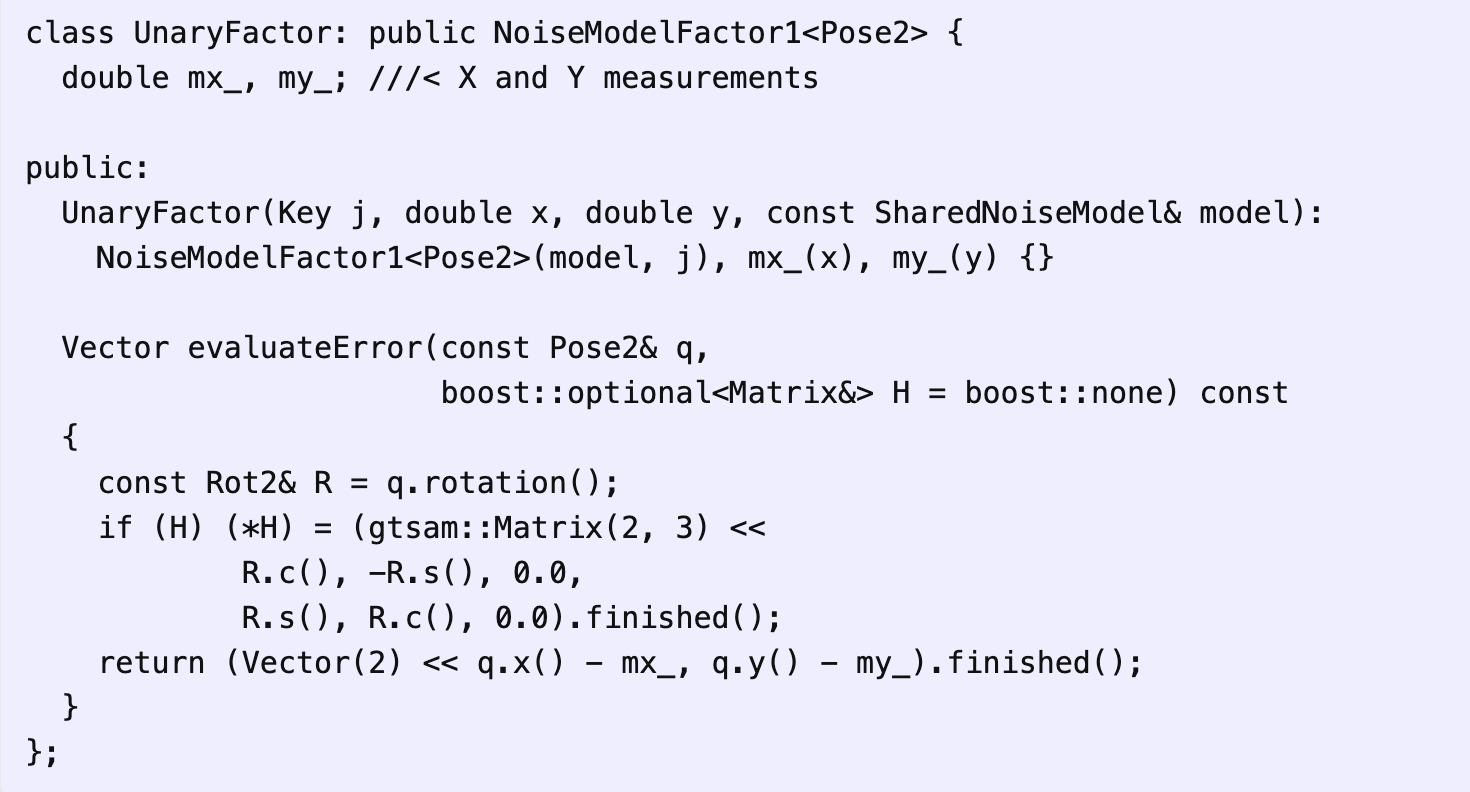
\includegraphics[width=10cm]{measurement-factor.png}}
\end{frame}

\begin{frame}{C++ Implementation - use of custom factors}
  \centerline{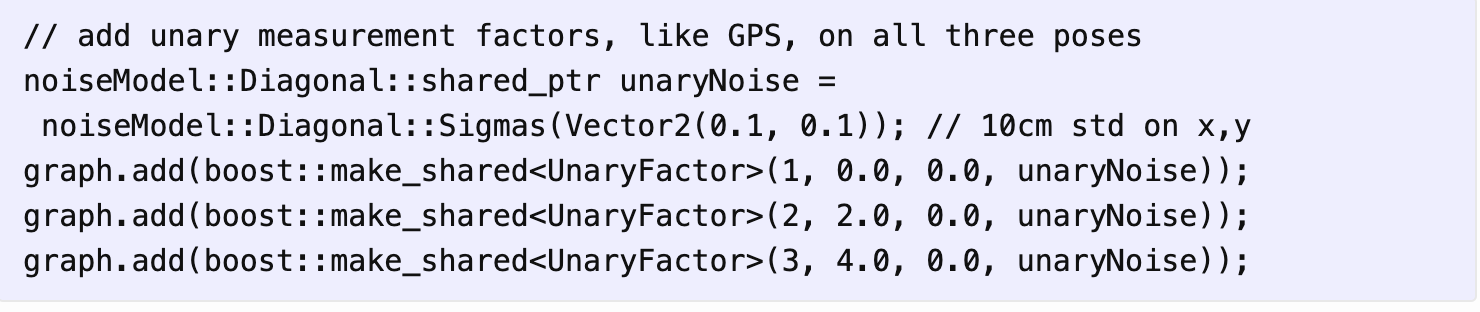
\includegraphics[width=10cm]{custom-factors.png}}
\end{frame}

\begin{frame}{Localization Results}
  \centerline{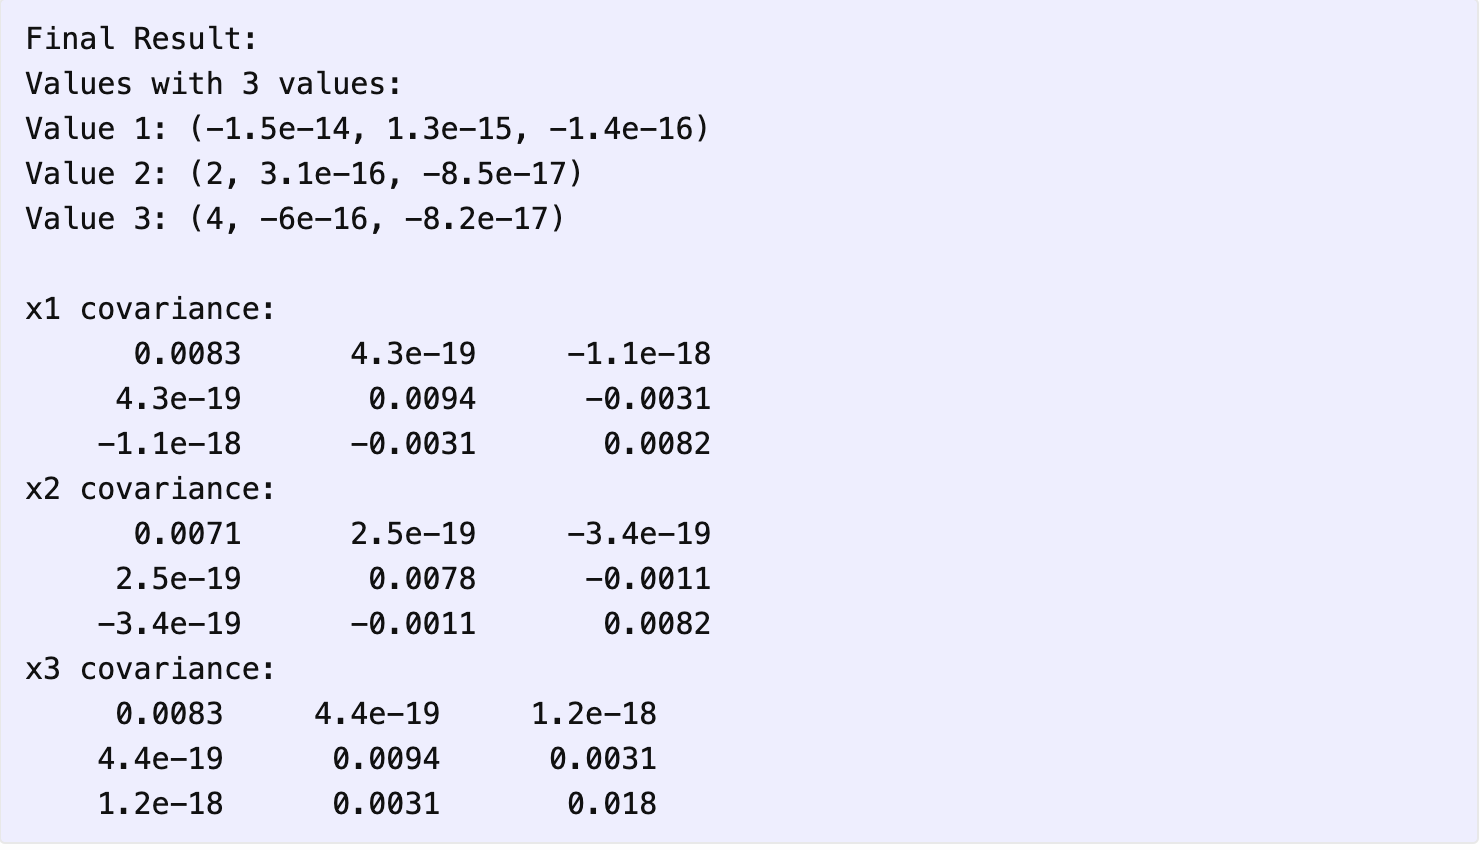
\includegraphics[width=10cm]{localization-results.png}}
\end{frame}

\begin{frame}
  \frametitle{Visualization of localization impact}
  $\begin{array}{cc}
    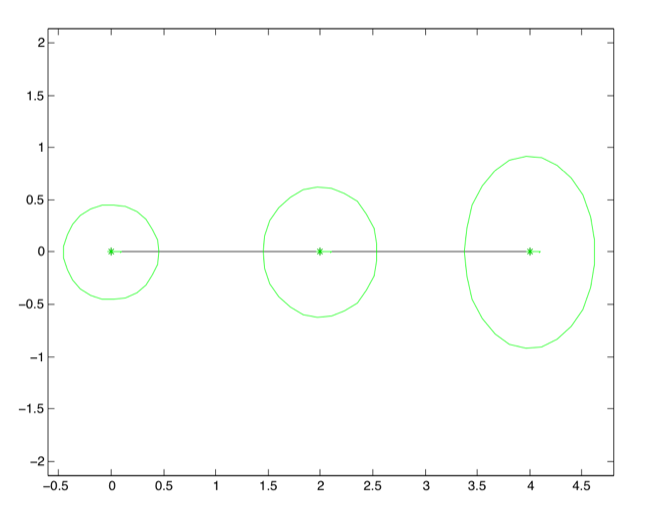
\includegraphics[width=5.5cm]{Odometry.png} &
    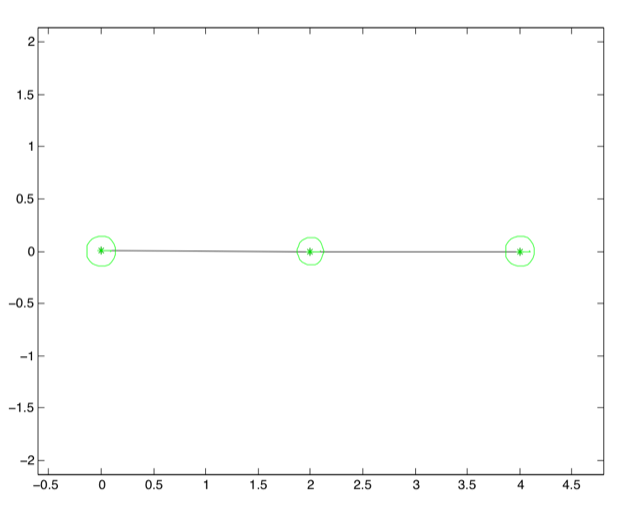
\includegraphics[width=5.5cm]{Localization.png}\\
    \mathrm{Odometry~~~results} &  \mathrm{Localization~~~results}\\
  \end{array}$
\end{frame}

\section{Pose SLAM}

\begin{frame}
  \frametitle{Pose SLAM}
  \begin{itemize}
    \item A simple way to combine multiple movements and measurements
    \item Well described in the literature (Durrant-Whyte et al. 1996)
    \item A key feature is loop closing. How to update when you return to a former location?
  \end{itemize}
  \centerline{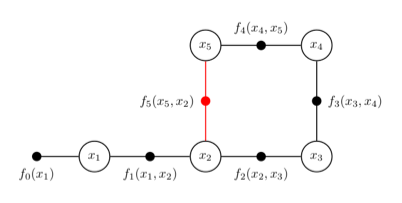
\includegraphics[height=5cm]{FactorGraph3.png}}
\end{frame}

\begin{frame}
  \frametitle{Loop closing}
  \begin{itemize}
    \item The estimation process is automatic, once you add the additional link
  \end{itemize}
  \centerline{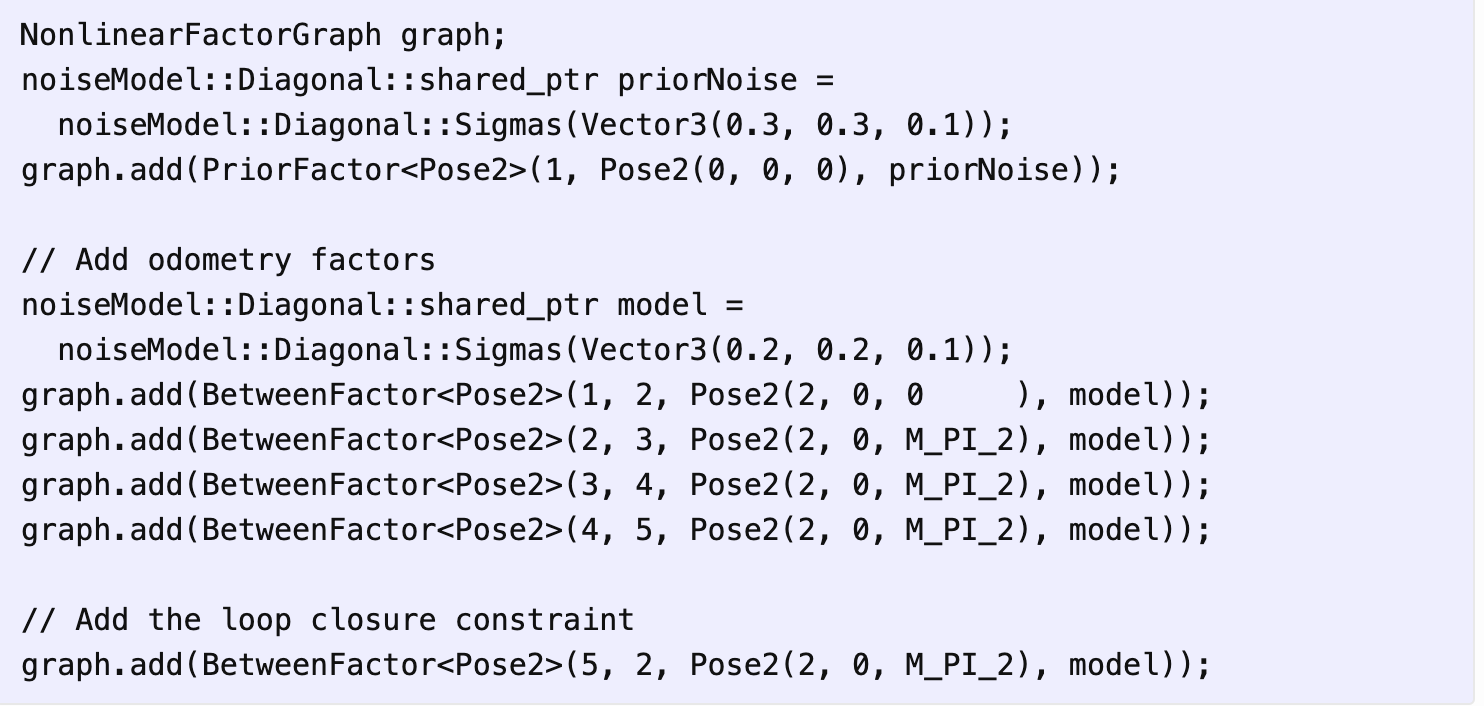
\includegraphics[width=10cm]{loopclosing-code.png}}
\end{frame}

\begin{frame}
  \frametitle{Estimation result with loop closing}
  \centerline{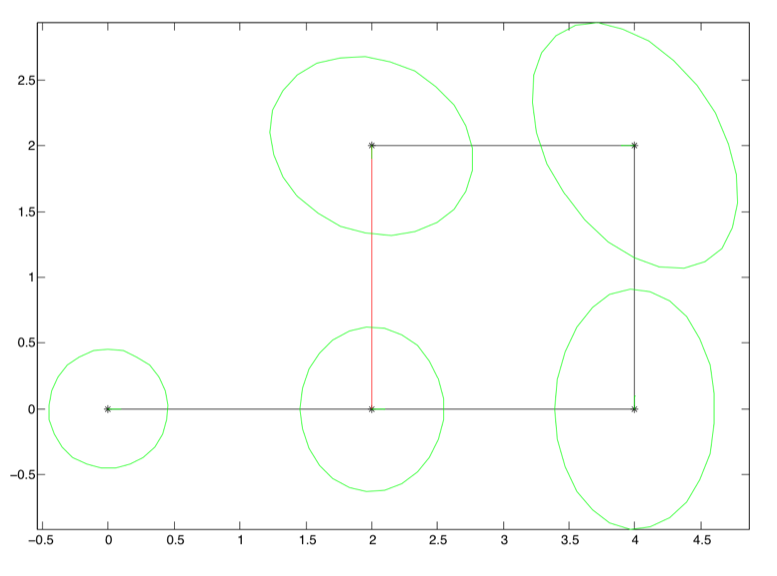
\includegraphics[width=9cm]{example1.png}}
\end{frame}

\begin{frame}
  \frametitle{Multiple languages wrapped for GTSAM}
  \begin{itemize}
    \item GTSAM has multiple language bindings such as Python, Matlab, \dots
    \item Small MATLAB example below
  \end{itemize}
  \centerline{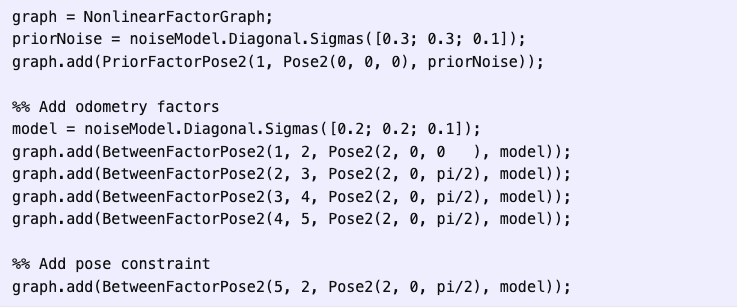
\includegraphics[width=10cm]{gtsam-poseslam-matlab.png}}
\end{frame}

\begin{frame}
  \frametitle{Small example}
  \centerline{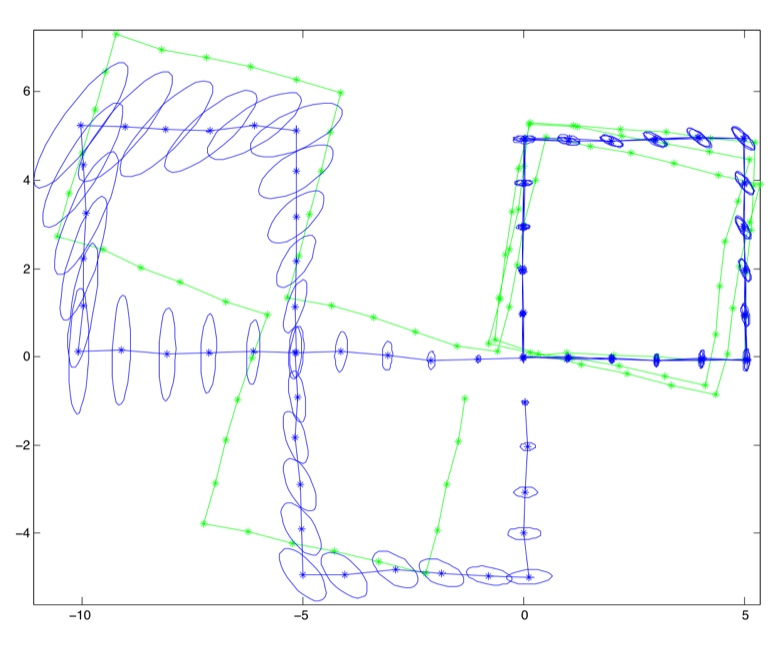
\includegraphics[width=9cm]{w100-result.png}}
\end{frame}

\begin{frame}
  \frametitle{Matlab code for the simple examaple}
  \centerline{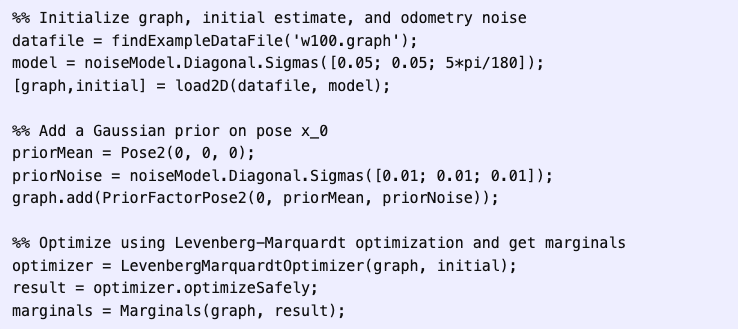
\includegraphics[width=9cm]{w100-matlab.png}}
\end{frame}

\section{Landmark-based SLAM}
\begin{frame}
  \frametitle{Landmark-based SLAM}
  \begin{itemize}
    \item In many applications we will have a well defined set of landmarks such as doors, windows, traffic signs, ... 
    \item We can use these landmarks as measurements to estimate the robot pose
    \item The same landmark may be seen multiple times or just a single time. 
  \end{itemize}
  \centerline{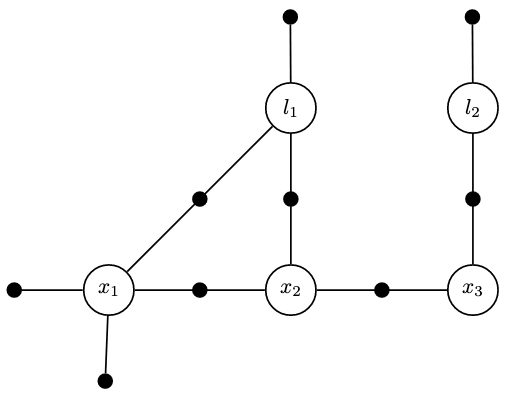
\includegraphics[width=8cm]{FactorGraph4.png}}
\end{frame}

\begin{frame}
  \frametitle{Estimation of the resulting graph}
  \centerline{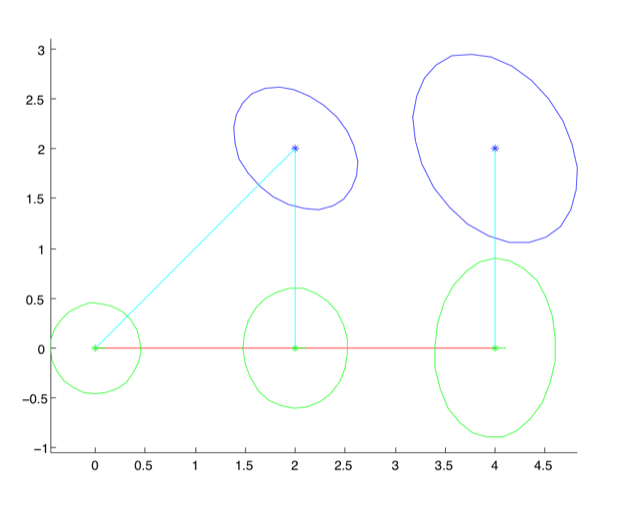
\includegraphics[width=9cm]{example2.png}}
\end{frame}

\begin{frame}
  \frametitle{Corresponding Matlab code}
  \centerline{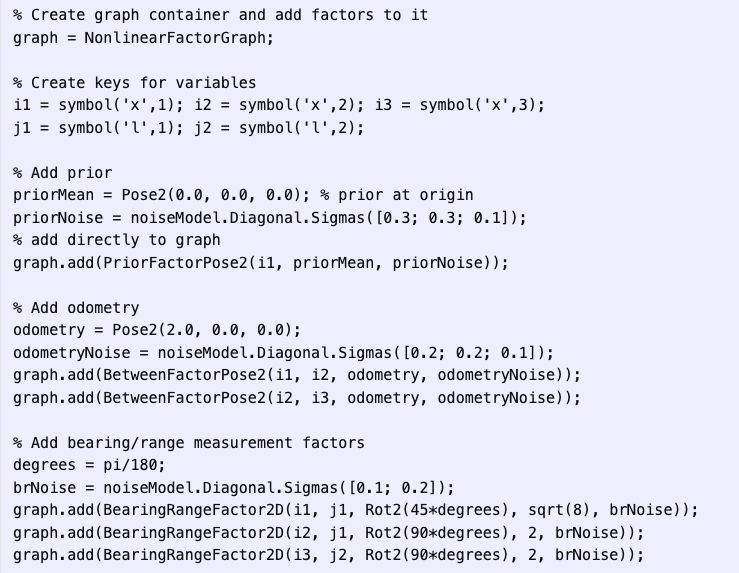
\includegraphics[width=8cm]{lms-matlab.png}}
\end{frame}

\begin{frame}
  \frametitle{Bigger example 1}
  \centerline{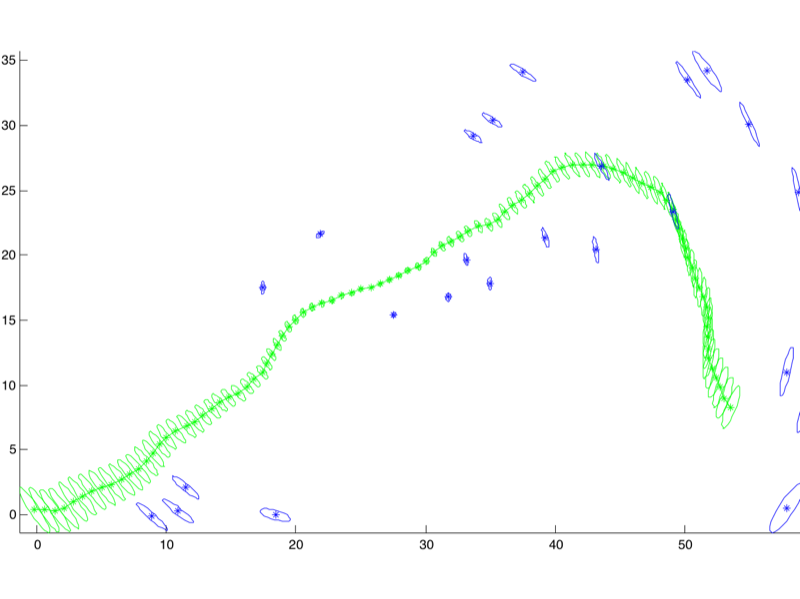
\includegraphics[width=10cm]{littleRobot.png}}
\end{frame}

\begin{frame}
  \frametitle{Bigger example 1 - Factor Graph}
  \centerline{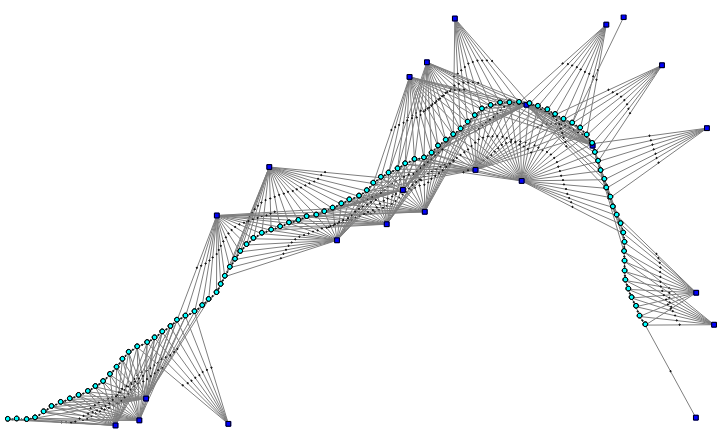
\includegraphics[width=10cm]{little-robot-factorgraph.png}}
\end{frame}

\begin{frame}
  \frametitle{Bigger example 2 - Victoria Park}
  \centerline{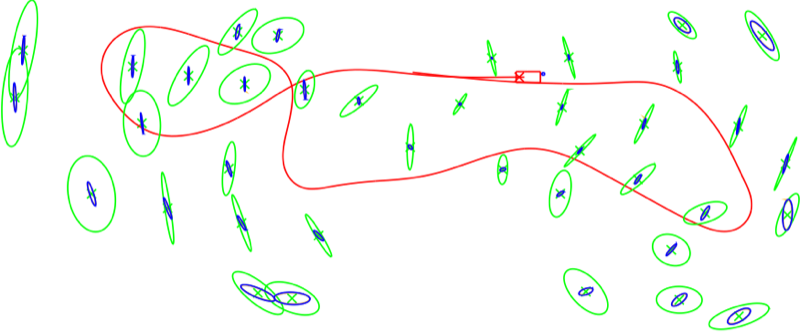
\includegraphics[width=10cm]{Victoria.png}}
\end{frame}

\begin{frame}
  \frametitle{Computing modes}
  \begin{itemize}
    \item SAM has multiple computing modes
    \item Full scale graph optimization
    \item iSAM which is incremental computing in real-time
    \item Tactonic SAM which is optimized for use of sub-maps
  \end{itemize}
\end{frame}

\begin{frame}
  \frametitle{Hierarchical Maps of MIT Strata Center}
  \centerline{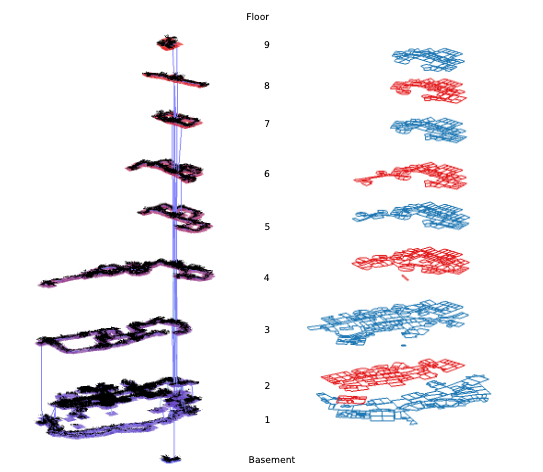
\includegraphics[width=8cm]{mit-strata-floors.png}}
  \centerline{The 10 floors of the MIT Strata Center}
\end{frame}

\begin{frame}
  \frametitle{Sample Map of MIT Strata Center}
  \centerline{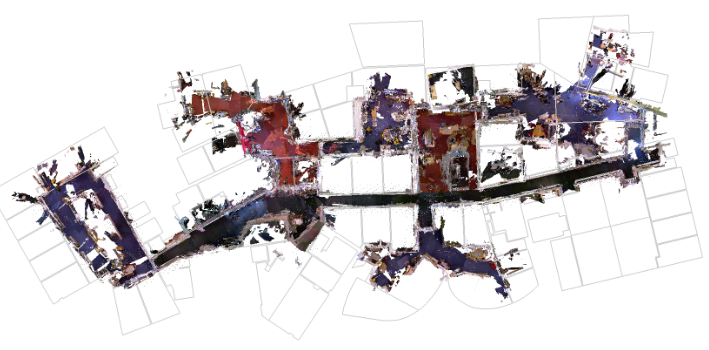
\includegraphics[width=8cm]{mit-strata-2nd-floor.png}}
  \centerline{The 2nd floor of the MIT Strata Center}
\end{frame}

\section{Summary}
\begin{frame}
  \frametitle{Summary}
  \begin{itemize}
    \item Factor graphs are a powerful tool for representing and solving estimation problems
    \item We exemplified its use with a set of examples for basic motion to
          integration of landmarks
    \item Today a very widely used tool for many problems in robotics
    \item Use by most major companies that do mapping and estimation
    \item Also widely used in computer vision for structure from motion challenge
    \item FNT paper gives a detailed view of the use-cases and underlying math
  \end{itemize}
  

\end{frame}
\end{document}

%%% Local Variables:
%%% mode: latex
%%% TeX-master: t
%%% End:
